\documentclass[tikz,border=7pt]{standalone}
\begin{document}
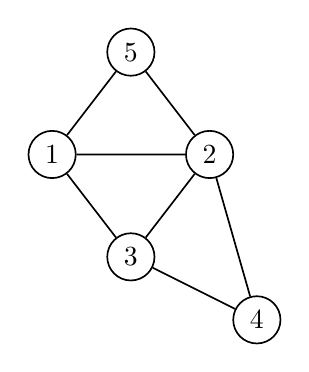
\begin{tikzpicture}[vertex/.style={draw,circle,minimum size=6mm,inner sep=0pt},line width=.6pt]
\node[vertex] (1) at (-1,1) {$1$};
\node[vertex] (2) at (1,1) {$2$};
\node[vertex] (3) at (0,-.3) {$3$};
\node[vertex] (4) at (1.6,-1.1) {$4$};
\node[vertex] (5) at (0,2.3) {$5$};
\draw (1)--(2) (1)--(3) (1)--(5) (2)--(3) (2)--(4) (2)--(5) (3)--(4);
\end{tikzpicture}
\end{document}
